\documentclass[11pt,letterpaper]{article}
\usepackage[top=1.00in, bottom=1.0in, left=1in, right=1.25in]{geometry}
\usepackage{graphicx}
\usepackage{latexsym,amssymb,epsf}
\usepackage{epstopdf}

\usepackage{sectsty,setspace,natbib}
\usepackage{float}
\usepackage{latexsym}
\usepackage{epsfig}
\usepackage{graphicx}
\usepackage{amsmath}
\usepackage{array}
\usepackage{lineno}
\usepackage{gensymb}
\usepackage{xr-hyper}
\externaldocument{phencc_supp}
% \usepackage{hyperref}

\usepackage{framed}

\linespread{1.1} % was 1.66 for double-spaced 
% \raggedright
\setlength{\parindent}{0.5in}
\pagestyle{empty}

\parskip=5pt
\pagenumbering{arabic}
\pagestyle{plain}
\setlength\parindent{0pt}

\begin{document}
\begin{flushright}
Version dated: \today
\end{flushright}
\bigskip
\noindent Running title: Environmental tracking 
% put in your own RH (running head)
\bigskip
\medskip
\begin{center}
% Insert your title:
\noindent{\Large {\bf How environmental tracking shapes communities in \\ stationary \& non-stationary systems}}\\
% Other titles: `Environmental tracking: It's more complicated than you think' (we hope) 
% or `Environmental tracking: Is it naive? Or, are we just naive?'
\bigskip
\noindent {\normalsize
E. M. Wolkovich$^{1}$ \& M. J. Donahue$^{2}$ }\\
\noindent {\small \it
$^1$ Forest \& Conservation Sciences, Faculty of Forestry, University of British Columbia, 2424 Main Mall, Vancouver, BC V6T 1Z4 (e.wolkovich@ubc.ca)\\
$^2$ Hawaii Institute of Marine Biology, University of Hawai`i at M\= anoa, K\=an`eohe, HI 96744 (donahuem@hawaii.edu)}\\
\medskip
\end{center}
\noindent{\bf Corresponding author:} see$^{1}$ above; Ph: 604.827.5246 (no fax).\\

\noindent \emph{Authorship statement:} EMW and MJD both conceived of the paper, performed modeling work and edited the paper, EMW additionally wrote the paper and did the literature review, while MJD additionally wrote the supplementary information on the model.  \\
\noindent \emph{Data statement:} Review, so no new primary data, but data from a comprehensive literature review will be archived in an appropriate public repository and the data DOI will be included at the end of the article. \\
\noindent \emph{Keywords:} community assembly, global change, climate change, phenology, environmental variability\\
\noindent \emph{Article type:} Reviews and Syntheses\\
\noindent \emph{Article information:} Abstract: 196 words; Main text: 5830; Figures: 4; Boxes: 3 (text in Box 1: 690; Box 2: 385; Box 3: 264); 93 references
% main text words (5500 without in-text refs approximately) 
\newpage
% \linenumbers % If you want to add need to add \begin{linenomath} and \end{linenomath} around all eqns (and check they still show up)

\begin{abstract} 
The modeling paper ... 
\end{abstract}


\begin{center}
\begin{table}
\begin{tabular}{ p{12 cm}  }
\hline \hline
\emph{Term--} and definition\\ % ADD figures!
\hline 
\emph{community assembly --}  \\
\emph{cue reliability --} the match between ideal timing and actual timing \citep{donald2013,bonamour2019} \\ 
\emph{environmental tracking --}  the phenological change due to an organism's cue system given change in the environment  (Fig. \ref{fig:defineET}, note the shift in timing between sites). For example, considering a tree where budburst is determined by a combination of chilling, forcing and photoperiod cues---its environmental tracking would the number of days shift in the timing of budburst in response to a change in environmental conditions, such as warmer winters and springs. \\ % By definition it includes any factors that cue an event; thus if an an herb produces flowers depending on sufficient light, temperature and soil nutrients, the that suite of cues ...
\emph{environment's variability --} which aspects of the environment vary, how (e.g., temporally each year, spatially at $x$ scale) and how much \\
\emph{equalizing mechanism --} \\
\emph{fundamental tracking --} there is an`ideal' timing that yields maximum fitness, and event timings moving away from this ideal result in reduced fitness \citep[a foundational concept of the trophic mismatch literature,][]{vissergienapp2019}.\\
\emph{non-stationary environment --} the underlying distribution of abiotic characteristics of a location (the major suite of characteristics varies by habitat type, but generally includes physical climatic factors, such as temperature and precipitation) is unchanged across time (i.e., constant mean and variance) \\
\emph{phenological cues --} \\
\emph{phenological events --} the outcome of a two-part process that is repeatedly observed over time. At each temporal unit, an event can either happen or not (when---part 1) and, if it happens, the event can vary in size or degree of investment (how much---part 2) \\
\emph{stabilizing mechanisms --} \\
\emph{stationary environment --} the underlying distribution of abiotic characteristics of a location changes over across time (e.g., warming temperatures, larger rainfall events)  \\
\emph{unpredictable --}  events that fall outside of those predicted by some model---in the case of environments, an unpredictable environment would be one where major abiotic characteristic(s) no distribution (stationary or non-stationary) or related model can adequately predict the future properties of those abiotic characteristic(s)   \\
\hline \hline
\end{tabular}
\caption{Glossary}
 \label{tab:gloss}
\end{table}
\end{center}

% START of USED to be in TRY TO ADD


Stationarity is common to much of the theory that underlies ecology, evolution, and myriad other research fields \citep[e.g.,][]{Milly:2008yu,nosenko2013}. 

\subsubsection{Future research in environmental tracking \& non-stationary systems}

[COULD ADD here something on how ecologists are bad at multivariate environments/joint distributions etc.] 

\section{Defining tracking}

As ideal timing is generally only clear in extremely simplified models or in retrospect, species often use environmental cues to attempt to predict and match their event timing to the ideal timing across environments in both space and time (Fig. \ref{fig:defineET}; this match between ideal timing and actual timing could be considered cue reliability). These cues combined with environmental variation define what we refer to as temporal environmental tracking (henceforth, `environmental tracking').

....

Environmental tracking is the change in the timing of key life history events in response to an organism's proximate environmental cues. It is a type of phenological tracking that is the outcome of fundamental tracking, and dependent on the intersection of the environment's variability and a species' proximate cues for the studied life history event. Further, the organism's cues will interact with environmental variability and, thus, under this definition, identical genotypes will have different tracking in different environments.

Each organism's set of cues forms the biological basis for how a species tracks, but measuring environmental tracking requires two more components.

The first component is the environment's variability...

Second, which aspect(s) of the environment researchers measure will determine `measured environmental tracking'. If researchers know the exact cue (e.g., a thermal threshold) or suite of cues (e.g., a interaction of thermal sums and daylength) and can perfectly measure these in an environment where the cue(s) varies, then an organism will track the environment perfectly. If researchers measure some related attribute (e.g., mean spring temperature in place of thermal sums) or only some of the organism's cues, then the organism will appear to track poorly (i.e., a noisier statistical relationship from poor measurement quality).  If researchers measure an environmental variable that is not directly related to the cue(s) that the species actually uses, but one correlated with it (e.g., an insect tracks daylength but researchers measure temperature) then they have not measured tracking per our definition.

Accurately measuring environmental tracking thus requires a complete knowledge of an organism's cue(s), the environment's variability and the relationship between the actual cues and measured environmental metrics. Knowing an organism's cues is inherently difficult, generally requiring a suite of experiments, process-based models and in-situ data to show that the model of cues is accurate. Not surprisingly then we lack this for almost all species, coming closest for some model species \citep[e.g., \emph{Arabidopsis thaliana},][]{Kingsolver2007,Wilczek:2009oa}, or species with very simple cues \citep[e.g., coral \emph{Acropora millepora},][]{levy2007} and have some basic information for some other species \citep[e.g., the Great Tit, \emph{Parus major},][]{charm2008}. 

\subsection{Measuring tracking}
Multiple meta-analyses now show plants' spring phenology shifts with spring or annual temperatures 4-6 days/$\degree$C on average across species \citep{Richardson:2006qh,Wolkovich:2012n,thackeray2016}, but also highlight high variation across species  \citep{Cook:2012pnas}, even after examining multiple major climate variables \citep{thackeray2016}. Variability across species appears similar when examining consumers tracking their prey \citep[across diverse species tracking over time is 6.1 days/decade but ranges from zero to 15 days/decade, see][]{kharouba2018}. 

\subsection{Tracking in single-species environments}
Applying these areas of research to environmental tracking, however, first requires understanding phenological events. In particular, while phenological events are often coded as on/off switches (e.g., a seed does/does not germinate; a coral does/does not spawn), they are almost always defined by investment decisions that are part of a continuous developmental process \citep{inouye2019}. 

Phenological events can be considered as the outcome of a two-part process that is repeatedly observed over time. At each temporal unit, an event can either happen or not (when---part 1) and, if it happens, the event can vary in size or degree of investment (how much---part 2). This process is generally applied at the level of the individual (but it could potentially apply at lower levels, for example buds on a branch, or potentially higher levels, such as all the offspring from a parent). Across time, it produces an event's distribution. After starting, many events are entrained to continue based on the underlying physiological process: for example, laying eggs within one clutch (here, the first part of the process is whether to lay eggs or not and the second is whether to continue to invest in that process, which would lead to additional eggs, which researchers then observe as number of eggs per temporal unit) or flowering each growing season. In such cases, first events at the individual-level are somewhat unique from the rest of the event's distribution. In all cases, these individual-distributions scale up to the population-level estimates of these events generally used by researchers \citep[see][for discussion of the outcomes of this scaling]{inouye2019}.

Considering the life history events that define part of environmental tracking as a two-part process highlights that tracking is ultimately shaped by resources that species need to grow and reproduce, and circles back to an organism's fundamental tracking. This is perhaps best recognized in the literature on trophic synchrony where there is often focus on how well consumers' environmental tracking matches to the seasonal distributions of their prey \citep{deacy2018,kharouba2018}. For example, decades of work has studied how birds (e.g., \emph{Parus major}) time their peak food demands---during their nesting season---to maximum prey (caterpillar) abundance \citep[e.g.,][]{charm2008}. Failure of environmental tracking to match prey year-to-year or over time with long-term warming has been tied to individual-level fitness consequences in some systems \citep{charm2008}, but not all \citep{visser2006}, which may be due to the complexity of mechanisms that influence total fitness \citep{Singer:2010eb,Johansson2012}. Environmental tracking in plants and other lower trophic levels is also about resources. Alpine plant species that emerge in step with snowmelt or temperature are likely responding, at least in part, to light resources for photosynthesis. Light equally appears critical to the sequence of phenology in many temperate forests: with lower-canopy species, and younger (shorter) individuals of higher-canopy species, routinely risking frost damage to leaf out before the canopy closes and access to light becomes severely reduced \citep{Vitasse2013,heberling2019}. These ultimate controllers on tracking---which determine fundamental tracking---are then filtered through the abiotic environmental cues species use to time events (Fig. \ref{fig:defineET}). From here, predicting tracking relates to predicting which cues an organism should use: an optimal control problem.% In both temperate as well as alpine systems, however, access to critical belowground resources also occurs in the spring---both for available water and for nutrients released with the turnover of seasonal microbial communities \citep{Zak:1990ar,edwards2010N}. Thus, plants' spring phenology in many systems is about careful tracking of nitrogen and other soil resources. As in higher trophic level systems, research has linked how well plants track to performance, with species that track warming tending to grow larger and/or produce more offspring \citep{Cleland:2012}.

\emph{Predicting variation in environmental tracking in stationary systems}\\
An optimal control framing can help predict which cues an organism should have based on a consideration of the costs, benefits, and constraints, in any one organism by environment system \citep{donahue2015}. First, it requires that benefits vary depending on the timing of event; this effect may be stronger in highly seasonal environments. Next, there must be a useful cue---some aspect of the environment that predicts resources or otherwise links back to the ultimate factors that shape environmental tracking \citep{gremer2016}. Some environments may inherently lack useful predictors, such as desert systems where few early-season variables seem to predict high or consistent rainfall years. 


\section{Future directions}
. To this aim, we review several major areas of research that we believe could most rapidly unite empirical and theoretical research in environmental tracking to advance the field.\\ % Including non-stationarity in ecological theory is non-trivial \citep{chessonnonstat,legault2019}, but is the current environment in which all observational ecology occurs.


...We expect progress will come from a balance between measures of fundamental tracking (measuring both event date variation and fitness), estimating an organism's system of cues (generally through controlled experiments followed by tests in the field), and measuring environmental tracking---that is the change in an event date from environmenatal variation that is due to cues. \R{r4miscvague} Clear statements of what is and is not known and measured will help. 


... Model interrogation can also use realistic environmental regimes to provide field predictions \citep{Wilczek:2010ad,Wilczek:2009oa} or predict future species and communities. One example of this comes from in silica resurrection experiments of model organisms where future environmental regimes included a mix of regular climate projections and projections modified to test and advance understanding of environmental tracking for the study species \citep[e.g., warmer winter and altered photoperiod scenarios in][]{fournier2016}.\\

\section{Box: What underlies variability in species tracking?}

% Predictability depends on the timescale of interest, which is related to a species' generation time \citep[which itself should be shaped by an environment and its predictability,][]{Davison2010,morris2008}. 

Accurately measuring environmental tracking depends on the temporal scale of the question (e.g., intra-annual versus inter-annual versus decadal), and how well researchers understand a species' underlying physiology and ecology. 

Thus, integrating tracking into these models requires fundamentally combining two different camps, which has not been done to our knowledge ... 

Models under this paradigm are generally composed of parameters that the describe the environment and the species within it. Parameters related to species must always include mechanisms for growth, death, interactions with other species, and generally a bet-hedging strategy for survival across years (e.g., a seedbank or other long-lived lifestage)---though exactly how these are defined varies across models.

% consider cost of static timing (cheap) versus tracking (potentially costly)
% Variation in tracking may also be predicted based on historical effects ... change in environment (species track old environment)
These include the costs to the organism of having a cue (or system of cues) to the environment (e.g., the machinery of monitoring temperature or daylength), the benefits of a cue (for example, how much tissue is saved by avoiding a coldsnap) and any constraints, such as cues that cannot be developed or evolutionary history making some cues more likely. 

\subsection{Interspecific variation in tracking}
% ADD  some numbers on variation in tracking ... why the variation? (1) it's hard to measure (keep this quick? Reference box?) and (2) maybe it's not always optimal to track
Despite the clear importance of tracking for resource access, 

Within populations, life-history can help predict how much individuals should track while also balancing trade-offs within and across seasons and years. Tracking has been repeatedly linked to fitness benefits \citep[e.g.,][]{farzan2018,deacy2018}. Such benefits usually break down into avoiding tissue loss or maximizing growth and, relatedly, maximizing reproduction. For species with bounded growing seasons, much literature has reviewed how tracking is a multivariate equation balancing early-season access to resources and its associated risks of tissue loss, with later season tracking of resources for reproduction and time for offspring to mature \citep{donohue2002,Morin:2005ye,Burghardt2015}. These trade-offs should also scale up to predictions of variation in tracking across species. % Species often track the start of growing seasons to avoid substantial tissue loss, for example from frost damage in temperate plants, or start activity only when resources for growth are present, such is the case in animals coming out of hibernation in cold regions. Equally, tracking of resources throughout a season is linked to the timing of reproduction for many species and, for iteroparous species, decisions on how much to invest each season requires estimating how likely a year is to be good for offspring.

These trade-offs with tracking, predicted by basic ecological theory and tentatively supported by growing empirical work, would have fundamental consequences for community assembly, especially with climate change. Applying ecological theory to current environments, however, is difficult because most theory has been developed for stationary systems, which are mathematically more tractable, but can sometimes be extended to non-stationary systems \citep{chessonnonstat}. Almost no community assembly research, however, has examined the consequences of shifting from a stationary to non-stationary environment. % Yet this transition is exactly what anthropogenic climate change has imposed on systems around the globe, making our understanding of how environmental tracking fits within community assembly theory critical. 
% .... that would have fundamental consequences for community assembly---at least in stationary systems. In non-stationary systems, theory is less developed for how tracking may trade-off with other traits (CITECHESSON), and even less theory predicts the consequences if the environment shifts from stationary to non-stationary

% How to explain warming experiments where researchers have identified links between performance and tracking, 
% links between tracking and performance in warming experiments could potentially wash out over longer timescales (fitness not measured over long enough timescales to consider diverse species life history strategies)

%  All these approaches  are focused on the proximate level---what environmental cues underlie tracking---at the ultimate level tracking is shaped by what resources species need to grow and reproduce. 
% The complex cueing mechanisms that drive environmental tracking interact with and shape patterns of resource acquisition and expenditure.”


\section{Tracking in multi-species environments}

% Lottery model: Birth and death rates vary ... collapses to single ratio (that's the environment) ... many general models are like this, they just vary a parameter and assume it is varying in response to the environment. Whatever parameter you allow to vary is how you allow the environment to filter through. (Side note: Tulja Purqur may have worked on how environment filters through to many species parameters in the model.)

.... priority effects 
% If one species is always early there has to be a trade-off. [Each year every species has a similar advantage and it's the same advantage every year, you could predict it with one year; in the other model the density effects are more variable by year -- you need inter-annual variation to predict the outcome. ]

 % Species that track in this model could be considered those that arrive earliest, however, priority effects generally require species that are highly similar to one another and thus models of priority effects do not predict variation in tracking across species, and further would not predict trade-offs between tracking and other traits \citep{fukami2015}. Trade-offs, however, are predicted from competition/colonization models: if species that track well are akin to species with high-dispersal, trackers may coexist by gaining early access to resources and reproducing before the later arrival of superior competitors.

% END of USED to be in TRY TO ADD


\newpage
\section{Main text} % Lizzie tried to only put text here that we did NOT use in the main text or supp of the (now primarily) review paper.




In the model, the population census of seeds, $N$, occurs at time $t$ at the end of the growing season (Equation 1).  Seeds survive over winter at rate $s$ and are lost from the population at rate $(1-s)$.  Surviving seeds germinate at rate $g_{i}(t)$.  Seeds that do not germinate remain in the seed bank until the next census at $t+1$.  Germination rate is a Gaussian function that declines with the distance between $\tau_{i}$, the species-specific preferred germination time, and $\tau_{p}(t)$, the timing of the resource pulse in year $t$, with maximum germination when $\tau_{i} = \tau_{p}(t)$ (Equation 6, Fig. \ref{fig:concept}a,b).  In cases that include tracking, the distance between $\tau_{i}$ and  $\tau_{p(t)}$ can be reduced by tracking, $\alpha_{i}$, resulting in greater germination fraction (Equation 7). \\

Germinating seeds are converted to seedling biomass at rate $b_{0}$ (Equation 4). Within year dynamics of the two species follows $R^{*}$ competition for a single resource.  The growing season begins with a single resource pulse $R_0(t)$.  Both  species consume the resource at rate $f(R)$ (Equation 3), and the resource undergoes abiotic loss (e.g., evapotranspiration) at rate $\epsilon$ (Equation 5).  Differences in $R^{*}_{i}$ were generated by differences in conversion efficiency, $c_{i}$. Species were otherwise identical in resource update parameters ($a$, $u$, and $\theta$) and in metabolic loss ($m$).  Biomass at the end of the season is converted into seeds at rate $\phi$, and the population of seeds is censused at $t+1$. \\

Interannual variation occurs in both the timing and the amount of the resource pulse.  The timing of the resource pulse varies from year to year and is given by $\tau_{p}(t)$, which is drawn from a $\beta$ distribution. The amount of resource available at the beginning of each season, $R_0(t)$, varies from year to year and is drawn from a log-normal distribution.  Each model run is comprised of a 500 year stationary period and a 500 year nonstationary period.  During the stationary period, $R_0(t)$ and $\tau_{p}(t)$ are each drawn from a stationary distribution.  During the nonstationary period, the timing of the resource pulse, $\tau_{p}(t)$, gradually shifts earlier in the season (Fig. \ref{fig:fig_Rt_tauPt}).  For the model runs displayed in Fig. \ref{fig:tauirstar} and Fig. \ref{fig:alpharstar}, this shift in the timing of the resource pulse is the only change in the environment during the nonstationary period.  We also discuss model runs in which the amount of resource, $R_0(t)$,  declines during the nonstationary period along with the shift in timing, $\tau_{p}(t)$ (Fig. \ref{fig:fig_Rt_tauPt}).  \\   

\subsubsection{Tracking in stationary environments}
Species must be sufficiently matched to their environment across years to persist for any long period of time. In our modeling framework, this means species must have a germination curve such that their effective biological start time ($\hat{\tau_{i}}$) is sufficiently close to the environmental start time ($\tau_{p}$) to allow germination of new seeds before the species' seedbank is exhausted. This can happen in effectively two ways: (1) species have fixed intrinsic biological start time values ($\tau_i$) close enough to the environmental start time ($\tau_p$; e.g., species A in Fig. \ref{fig:concept}b) to persist, or (2) species have a combination of an intrinsic biological start time ($\tau_i$) and tracking ($\alpha$) that brings the species' effective biological start time ($\hat{\tau_{i}}$) close enough to the environmental start time (e.g., see species B in Fig. \ref{fig:concept}b) to persist.  

A simple outcome of this model is that in temporally variable environments where all other species characteristics are identical, the species with the effective biological start time closest to the average environmental start time will always win---regardless of whether this effective biological start is due to a fixed intrinsic start time or due to tracking (or some combination of the two). Put another way, in a stationary environment both tracking and a fixed intrinsic start time are equally useful ways to match to the environment---all that matters is the effective distance between the biological and environmental start of the season. This is because both represent the same niche axis---the temporal niche. 

% (A large chunk of this is in review paper as of 21 Feb 2020.) As both a fixed intrinsic start time and tracking represent the same major niche axis, species cannot coexist given only variation in these traits---coexistence requires variation in another trait axis. As discussed above, theory and empirical work suggest this trade-off may involve traits related closely to resource competition. With this added variation---here we varied species' $R^*$ (via $c_i$)---species can persist together as long as those species with a temporal niche advantage are also the inferior competitors (Fig. \ref{fig:tauirstar}-\ref{fig:alpharstar}). That is, species that can draw resources down to a lower level and are thus the superior within-season resource competitors (lower $R^*$) can persist with species with that are inferior competitors but have realized biological start times closer to the environmental start time (regardless of whether that realized biological start time is a result of a fixed trait or tracking)---a finding inline with currently observed empirical trade-offs (see Box `Trait trade-offs with tracking'). These trade-offs, however, are all environmentally dependent. They hold only so long as the environment is stationary. 



\subsubsection{Tracking in non-stationary environments}

The two species coexistence model (see Equations 1-6 above) includes both interannual variation in the environment and intra-annual resource competition.  The model was modified from \citet{Chesson:2004eo}, which was originally conceptualized for annual plants with a seedbank.  Although the model can be conceived of more generally, we use the language of annual plant germination for concreteness.  

In communities where species traded-off competitive traits ($R^*$) with non-trackers---species with fixed intrinsic biological start times ($\tau_i$)---species with earlier start times were clearly favored in the non-stationary environment, generally driving the other species (with a lower $R^*$ and later start time) extinct before the end of our 500 year time-period (Fig. \ref{fig:tauirstar}). Very few two-species communities persisted through the end of the non-stationary period (2 out of 547 two-species communities persisting after end of stationary, or 0.04\%); those that persisted did so because the strong similarity between the two species slowed competitive exclusion (i.e., the two species were nearly identical in both $R^*$ and intrinsic biological start time, $\tau_i$). These species were thus persisting mainly through equalizing mechanisms. In the previous stationary environment species coexisted through both equalizing and stabilizing mechanisms, but the stabilizing mechanisms were lost in the non-stationary environment, as the system shifted away from the region of the temporal niche axis that the communities formed in. 
% Very few two-species communities persisted through the end of the non-stationary period (2 out of 547 two-species communities persisting after end of stationary, or 0.04\%) and those that did were generally persisting via being highly similar---having nearly identical $R^*$ and fixed intrinsic biological start time traits ($\tau_i$). These species were persisting through equalizing mechanisms---by being almost the same neither species could drive the other extinct, though these species do not coexist (as in longer simulations one species would be lost through drift or related mechanisms). The contrast of equalizing mechanisms---stabilizing mechanisms---include niche differences, such as the trade-off in competitive traits ($R^*$) with a fixed intrinsic biological start time trait ($\tau_i$). Yet, in this non-stationary system stabilizing mechanisms failed to yield any persistence of two-species communities as the environment shifted away from the previous trade-off axis the communities formed in. 

Persistence of two-species communities via both stabilizing and equalizing mechanisms occurred more often in communities where species traded off competitive traits ($R^*$) with tracking ($\alpha$). 
...
Tracking, in contrast to fixed biological start times, allowed the species with the competitive advantage in effective start time to shift along the temporal niche axis as the environment shifted.  


\subsubsection{Model conclusions}

While in stationary systems both tracking and a fixed intrinsic start time can allow a good match to the environment, tracking is superior as environments shift to non-stationarity, confirming the current paradigm that climate change favors species that track the environment. 

Our model, however, makes a number of assumptions about how species respond to non-stationarity in the environment. We imposed environmental non-stationarity on an axis fundamental to coexistence. Yet, non-stationarity in the environment can take on many forms---both in what variable it affects and how it reshapes the underlying distribution of that variable. Communities that assemble via other axes of the environment than start of season timing may be far less impacted than our simulations suggest. Further, we examined a common trend with climate change---shifts in the mean of the environment. Changes can also occur in the variance or the fundamental shape of the distribution (e.g., shifting from a normal distribution to one that is more similar to a Gamma). Additionally, we applied a shift to only one aspect of the environment. In reality, climate change may impose multivariate shifts.

Human modification of the globe imposes complex shifts in the environments of most species. If the environment shifts along multiple niche axes involved in community assembly, it may allow trade-offs that structure communities to persist through non-stationary periods. We examined this possibility by again shifting the mean start of season earlier (i.e., changing the temporal niche) and, at the same time, decreasing the mean size of the resource pulse by half (i.e., changing the resource niche). Thus, our environment simultaneously favored species with earlier start times and superior within-season competitive abilities (lower R*). We found little evidence, however, of communities persisting via a maintained trade-off---instead the inherent variability of a system shifting in two dimensions drove species extirpations higher (14.8\% of two-species communities remaining after non-stationary). Thus, while a multivariate nonstationary environments may, in principle, maintain trade-offs, the shifts in the joint distribution would need to be so balanced that it seems unlikely. More likely appears the possibility that multivariate shifts in the environment make species more vulnerable to local extirpation \citep{sixthectinction2011,IPCC:2014sm}.


%=======================================================================
% References
%=======================================================================
\newpage
\bibliography{/Users/Lizzie/Documents/git/bibtex/LizzieMainMinimal}
\bibliographystyle{/Users/Lizzie/Documents/git/bibtex/styles/ecolett.bst}


%=======================================================================
% Tables
%=======================================================================

%\begin{center}  
%\begin{table}
%\caption{Key differences between PWR and traditional PCMs such as PGLS.}
%\begin{tabular}{ | p{4cm} | p{5.5 cm} | p{5.5 cm} |}   \hline 
%& PWR & PCMs (e.g., PGLS) \\ \hline \hline
%Major goal & Study of evolution of correlation between variables across species & Study of evolution of correlation between variables across species\\ \hline
%\emph{Assumption 1:} Nature of correlation between two or more variables & Non-stationary (changes through phylogeny in a phylogenetically conserved fashion) & Stationary (constant) throughout phylogeny (all variation is noise) \\ \hline
%\emph{Assumption 2:} Completeness of variables & Substitutes phylogeny for variables (simple or complex) not in the model that interact with variables in the model & Assumes variables in model are primary drivers of correlational relationship \\ \hline
%Inferential mode & Usually exploratory & Hypothesis testing (statistical significance)\\ \hline
%Outputs & Coefficients of regression changing through the phylogeny & p-value and single set of coefficients presumed to apply to entire phylogeny with their confidence intervals\\ \hline

%Method to avoid overfitting & Cross-validation (boot-strapped determination of optimal band-width for accurate prediciton of hold-outs) & Exact analytical model of errors and degrees of freedom\\ \hline \hline
%\end{tabular}
%\end{table}
%\end{center}

%=======================================================================
% Figures
%=======================================================================
\clearpage


\begin{figure}[t!]
\centering
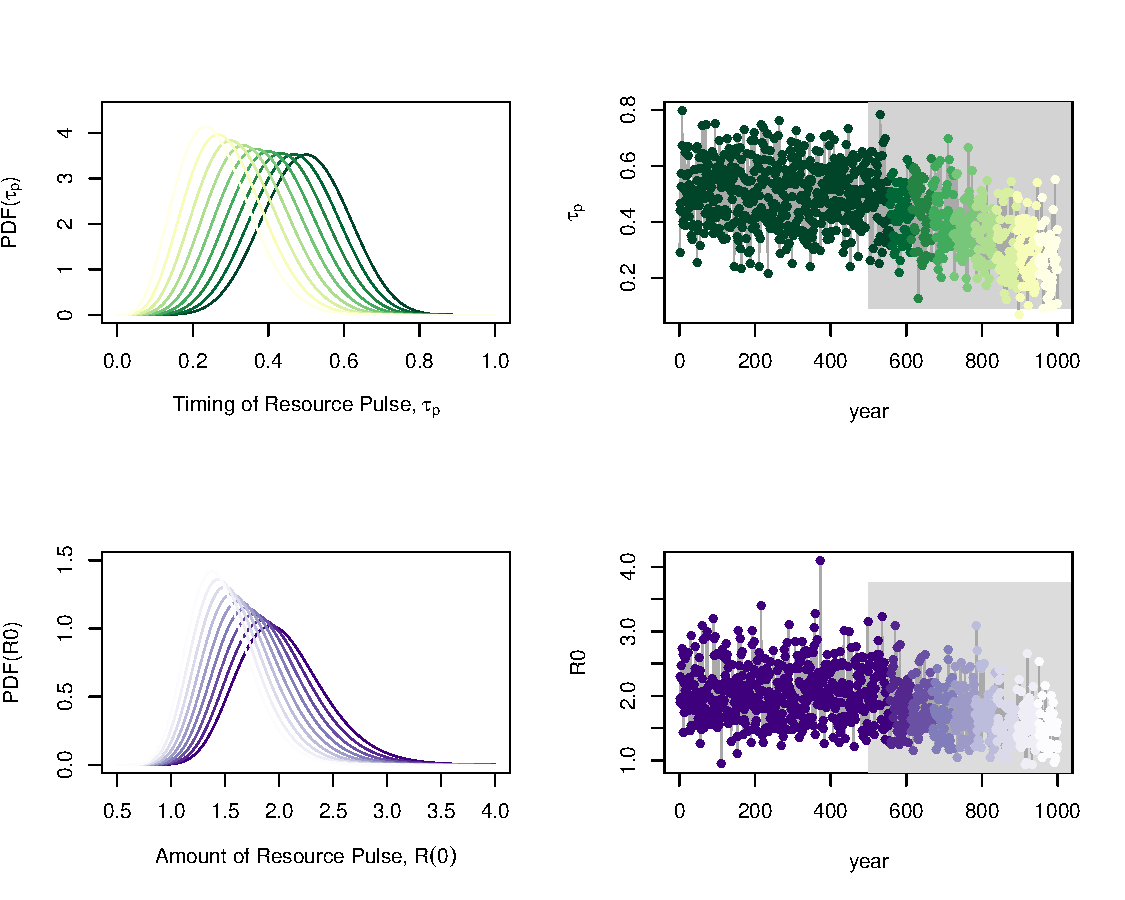
\includegraphics[width=1\textwidth]{..//..//R/graphs/modelruns/manuscript/modelsupp4panel.pdf}
\caption{How the environment shifts from the stationary period to the nonstationary period. The timing of the resource pulse shifts from $\tau_{p} \sim \beta(10,10)$ for the 500 year stationary period to $\tau_{p}$ \sim $\beta(5,15)$ over the 500 year nonstationary period.  For simulations where the amount of resource is also changing, $R(0)\sim logNormal(log(2), 2))$ during the 500 year stationary period and shifts to $R(0) \sim logNormal(log(2)/2,2)$ during the nonstationary period.}
\label{fig:fig_Rt_tauPt}
\end{figure}

\begin{figure}[t!]
\centering
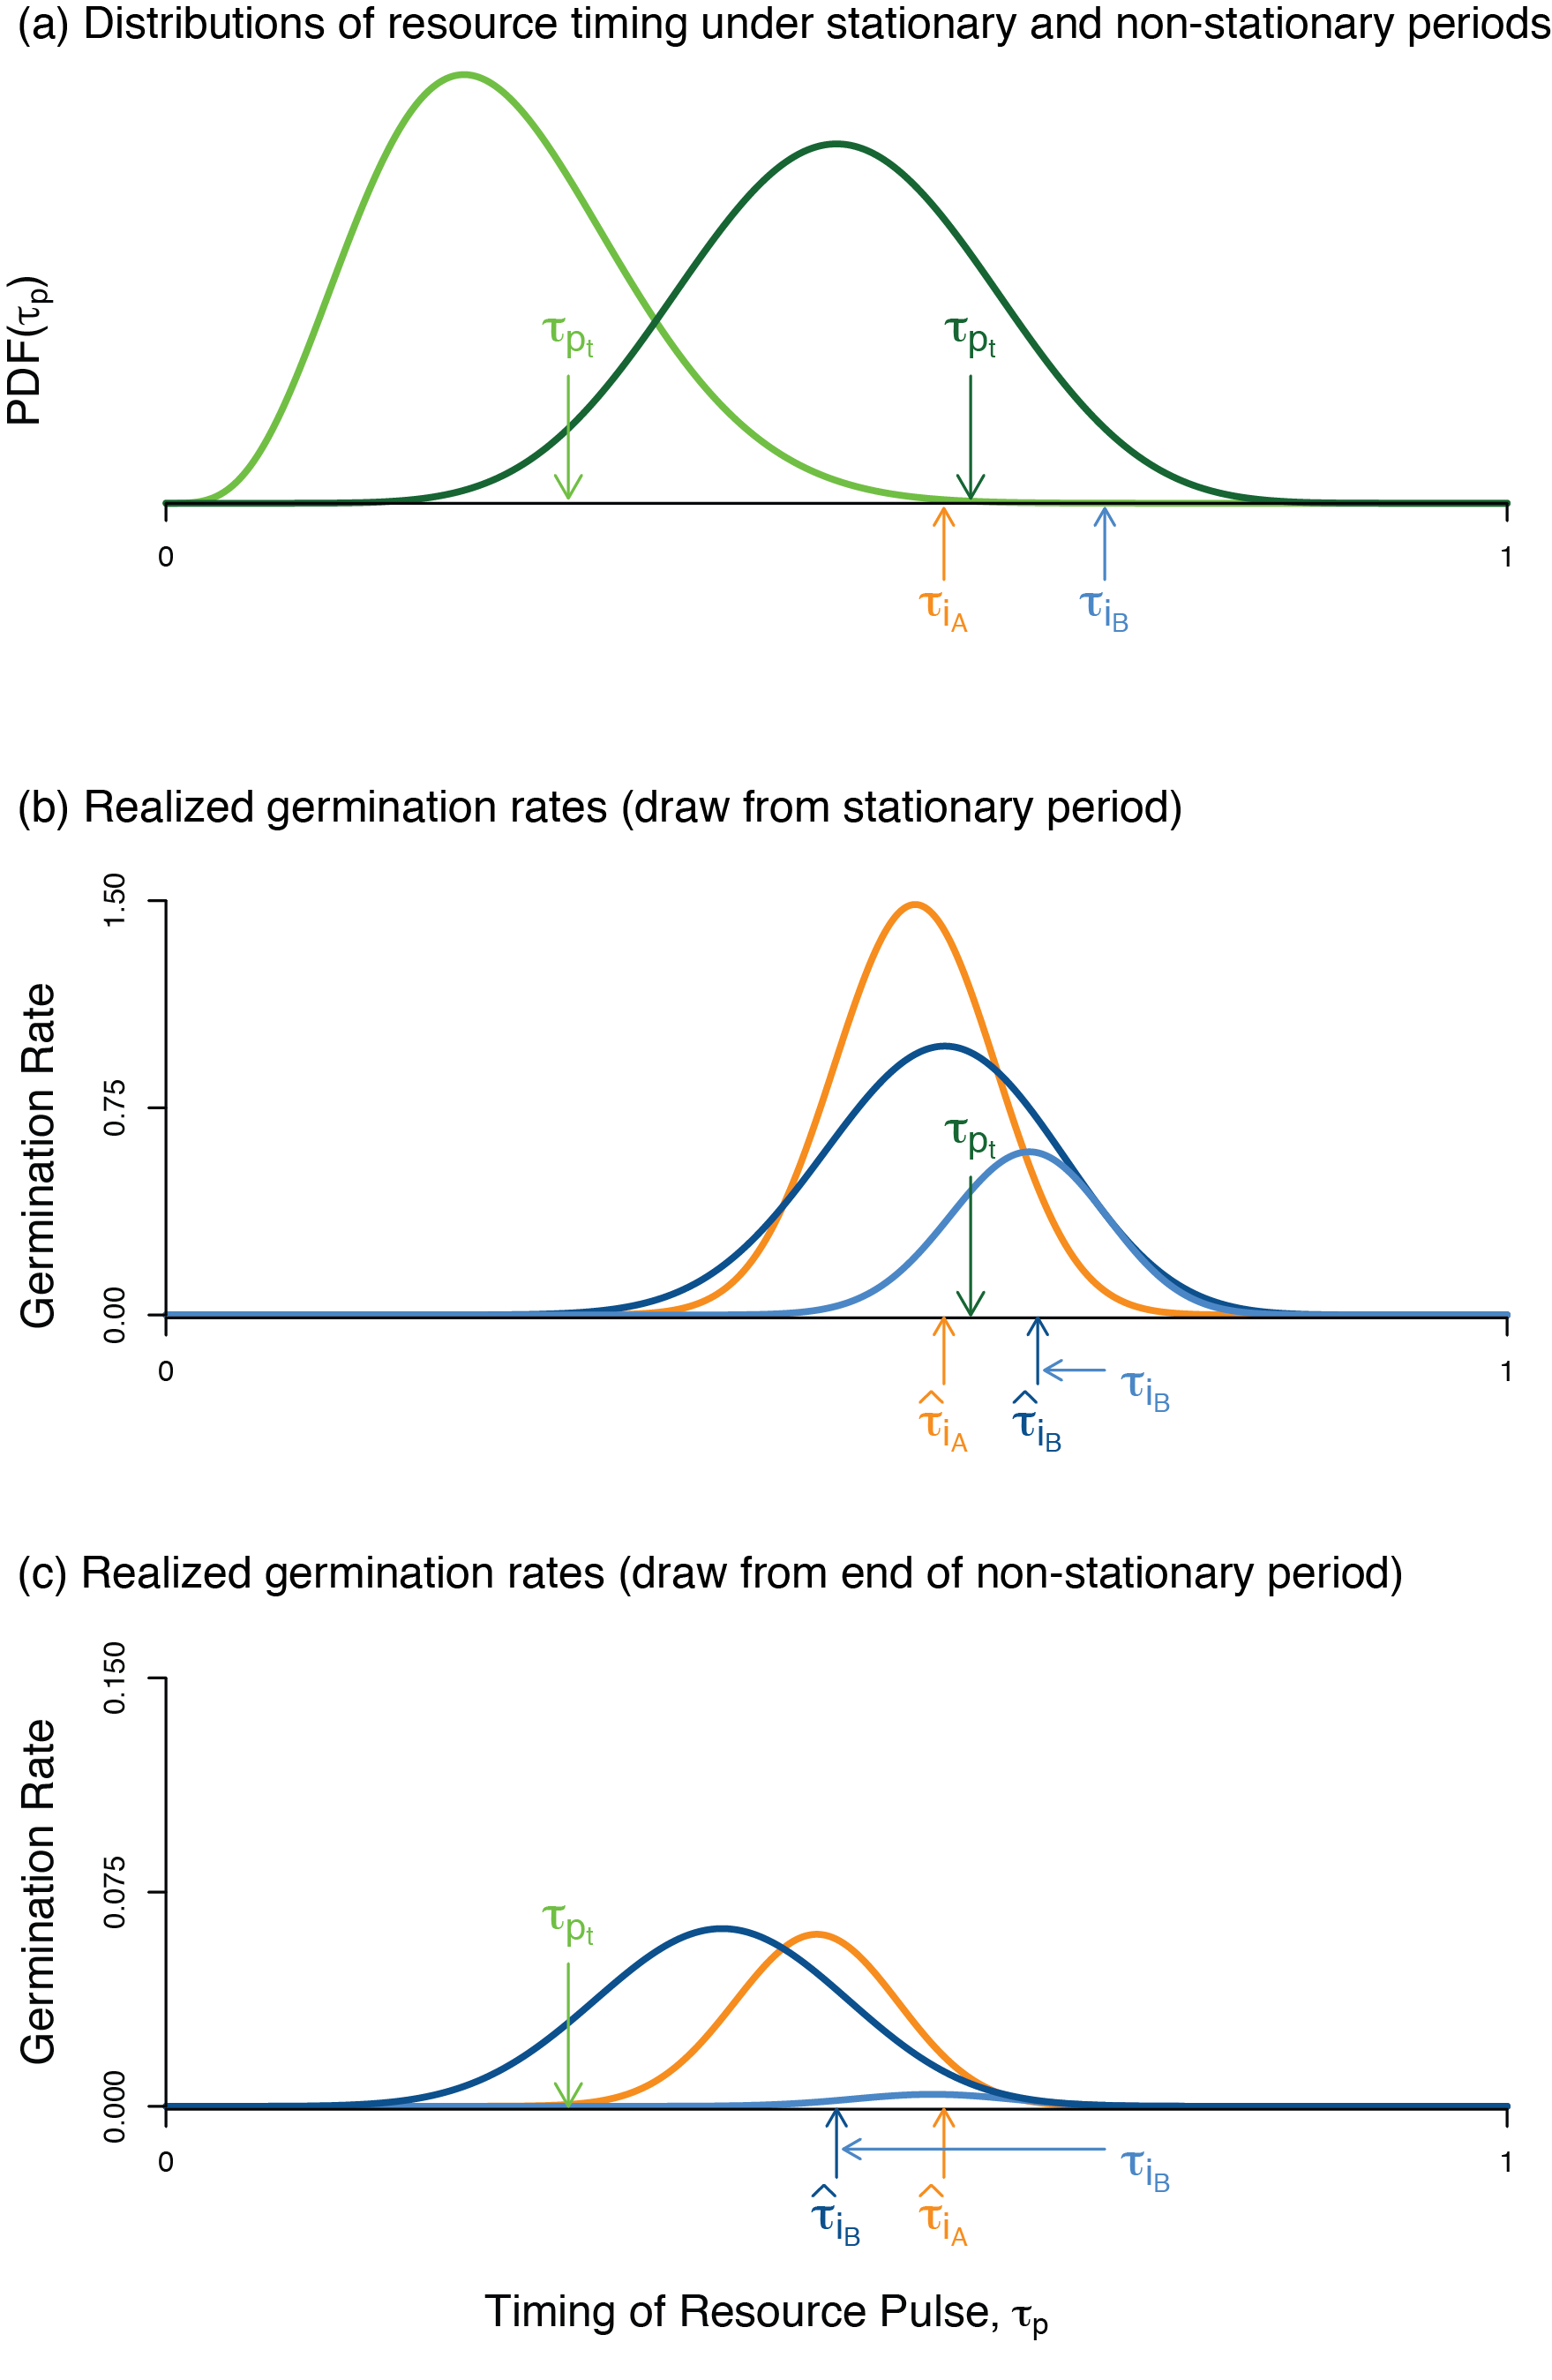
\includegraphics[width=0.65\textwidth]{..//..//R/graphs/conceptual/TauP_GerminationAdj.png} 
\caption{The distributions of the environment (a) and species' germination for two sample years (b-c) in our seed germination model. (a) The timing of the resource pulse ($\tau_p(t)$), which defines the environmental start of season, is $\beta$-distributed with parameters $\beta(10,10)$ during the stationary period (dark green) shifting to $\beta (5,15)$ through the nonstationary period (light green). (b) Realized germination rate as a function of $\tau_p(t)$ for two species during the stationary period: the orange line is a non-tracking species A with preferred germination time, $\tau_{iA}$, that is close to the mean of the stationary period; the blue lines show the difference in realized germination rate of a tracking species with a preferred germination time, $\tau_{iB}$, that is further from the mean of the stationary period both without (light blue) and with (dark blue) the effect of tracking; note the shift from $\tau_{iB}$ to $\hat{\tau_{iB}}$. (c) Realized germination rate of species A and species B at the end of the nonstationary period. Note the change in axes from (b) to (c) shows the decline in overall germination rate as the environment moves away from the preferred germination time of both species.} % I'm not sure that "realized germiantion" is the best phrase, but it is the germination rate given tauP times the prob of tauP under that STA or NST period.  So it it he realized germination rate for each species given the environment.  
% If, in a particular year, $\tau_i$ is close to $\tau_p$, a large fraction of species $i$ seeds will germinate (e.g., Fig. \ref{fig:concept}b) ; if $\tau_i$ is far from $\tau_p$, a small fraction of the seeds will germinate.  Figure \ref{fig:concept} b-c illustrate the germination rate of two species with different $\tau_i$ values under two different environments.   

\label{fig:concept}
\end{figure}
%% Figure reference to the supplement isn't working in the caption for Figure 3 or 4!
\begin{figure}[t!]
\centering
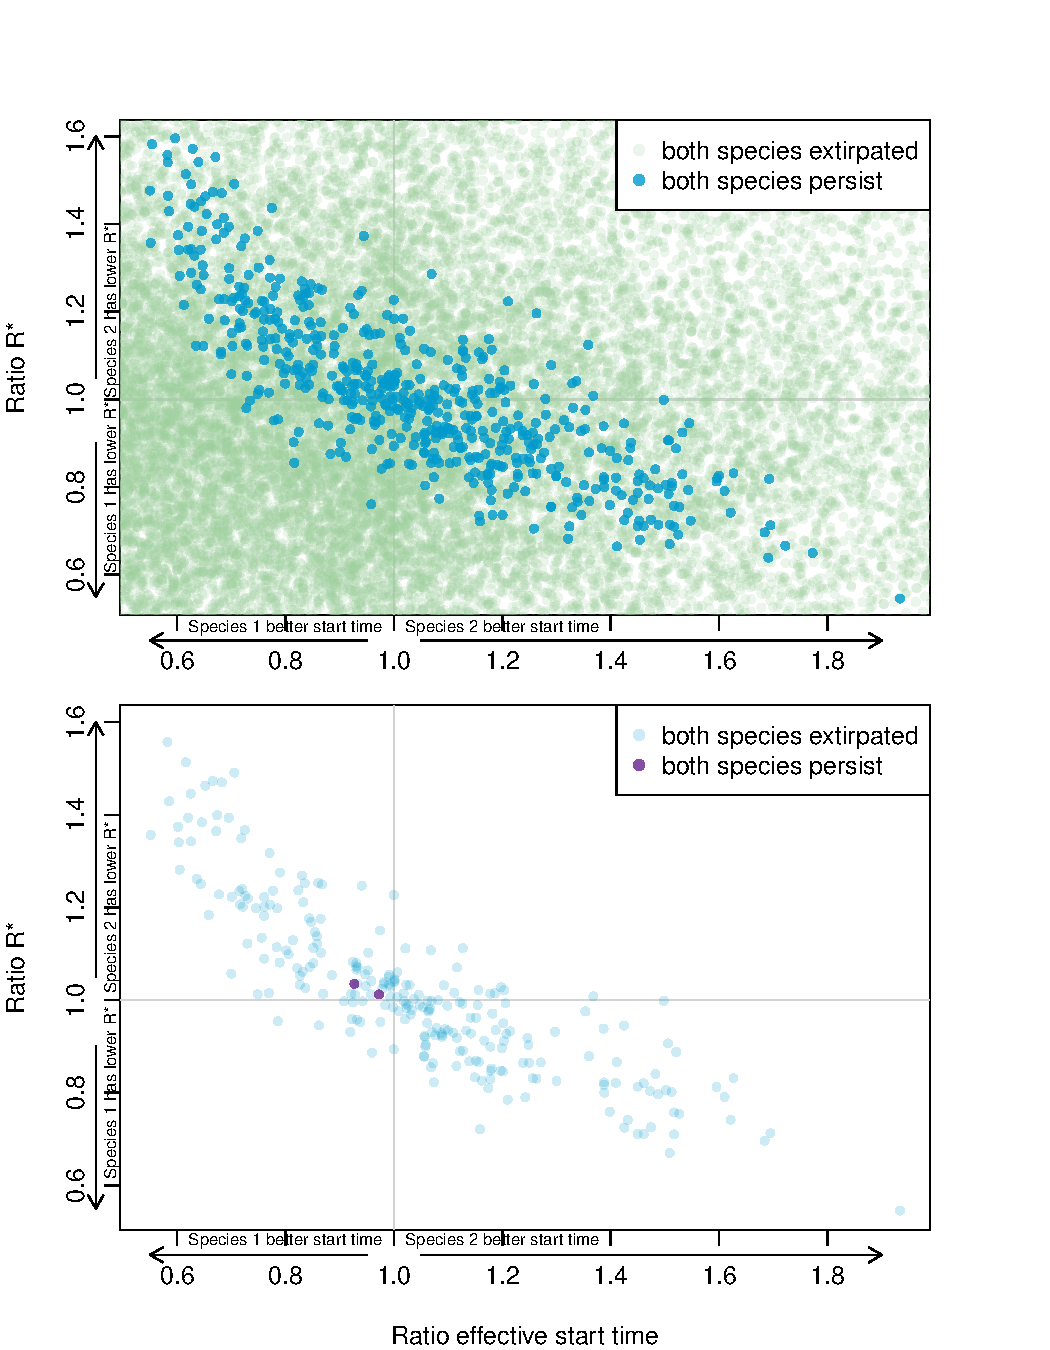
\includegraphics[width=0.9\textwidth]{..//..//R/graphs/modelruns/manuscript/tauIPrstart1_2panel.pdf}
\caption{How non-stationarity reshapes two-species communities in a simple model where effective start time (X axis: species 1/species 2) trades off with $R^*$ (Y axis: species 1/species 2): each point represents one two-species community color-coded by whether both species persisted or one or more species was extirpated through 500 years of a stationary environment (top), followed by an additional 500 years of non-stationary environment (bottom), where the abiotic start of the season shifts earlier. Only two-species communities that persisted through the stationary period are shown in the bottom panel. See Fig. \ref{fig:tauirstarsupp} for an alternative version of this figure detailing one-species outcomes.}
 \label{fig:tauirstar}
\end{figure}


\end{document}
%%%%%%%%%%%%%%%%%%%%%%%%%%%%%%%%%%%%%%%%%%%%%%%%%%%%%%%%%%%%%%%%%%%%%%%%
